%hallo
\documentclass[english, % Standardmäßig deutsche Eigenarten, englisch -> english
parskip=full, % Absätze durch Leerzeile trennen
bibliography=totoc, % Literatur im Inhaltsverzeichnis
%draft, % TODO: Entwurfsmodus -> entfernen für endgültige Version
]{scrartcl}
\usepackage{ifluatex} % zum Testen, ob LuaTeX verwendet wird
\ifluatex
\usepackage{fontspec} % Laden von Schriften
\setmainfont[Mapping=tex-text]{Linux Libertine O}  % Mapping ermöglicht die Verwendung z.B. von --
\setsansfont[Mapping=tex-text]{Linux Biolinum O}
\usepackage{polyglossia}  % Sprachpaket
%\setdefaultlanguage[spelling=new,babelshorthands=true]{german}  % Neue Rechtschreibung und Abkürzungen
\else % kein LuaTeX
\usepackage[utf8]{inputenc} % Kodierung der Datei
\usepackage[T1]{fontenc} % Vollen Umfang der Schriftzeichen
\usepackage{lmodern}
%\usepackage[ngerman]{babel} % Sprache auf Deutsch (neue Rechtschreibung)
%\usepackage{libertine} % Schriftart Linux Libertine/Biolinum verwenden
\fi

% Mathematik und Größen
\usepackage{amsmath}
\ifluatex
\usepackage{unicode-math}
\fi
\usepackage[locale=US, % deutsche Eigenarten, englisch -> US
separate-uncertainty, % Unsicherheiten seperat
]{siunitx}
\usepackage{physics} % Erstellung von Gleichungen vereinfachen

% Bilder einbinden
\usepackage{graphicx}
\usepackage{float}
\usepackage{caption}
%\graphicspath{{bilder/}} % TODO: Pfad unter dem die Bilder gesucht werden

% Gestaltung
\usepackage{microtype}  % Mikrotypographie
\usepackage{booktabs}  %schönere Tabellen
\usepackage[toc]{multitoc}  %mehrspaltiges Inhaltsverzeichnis
\usepackage{csquotes} % Anführungszeichen mit \enquote
\usepackage{subfigure}  % Unterabbildungen a,b,c,…
\usepackage{enumitem}  % Listen anpassen
\setlist{itemsep=-10pt}
\usepackage{scrpage2}  % Manipulation des Seitenstils
% Kopf-/Fußzeilen
\pagestyle{scrheadings}
\clearscrheadings
\automark{section}
\ofoot{\pagemark}
\ihead{\headmark}
\setheadsepline{.5pt}

\usepackage[colorlinks=true]{hyperref}  % Links und weitere PDF-Features

\makeatletter 
\renewcommand\subsection{\@startsection 
   {subsection}{2}{0mm}%      % name, ebene, einzug 
   {0.5\baselineskip}%            % vor-abstand 
   {0.3\baselineskip}%            % nach-abstand 
   {\bfseries\sffamily\large}%           % layout 
   } 
\makeatother 

% TODO: Titel und Autor, … festlegen
\newcommand*{\titel}{Biomolecular Motors: From Cellular Function to Nanotechnology}
\newcommand*{\autor}{Maximilian Obst, Thomas Adlmaier}
\newcommand*{\abk}{MMC}
\newcommand*{\betreuer}{M.Sc Matthäus Mittasch}
\newcommand*{\messung}{21.10.2016}
\newcommand*{\ort}{Max Planck Institute of Molecular Cell Biology and Genetics}

\hypersetup{pdfauthor={\autor}, pdftitle={\titel}} % PDF-Metadaten

\titlehead{F-Praktikum \abk \hfill TU Dresden}
\subject{Experiment protocol}
\title{\titel}
\author{\autor}
\date{\begin{tabular}{ll}
Protocol: & \today\\
Measurement: & \messung\\
Place: & \ort\\
Tutor: & \betreuer\end{tabular}}

%----------------
\begin{document}
\begin{titlepage}
\maketitle

\begin{figure}[hb] 
  \centering
     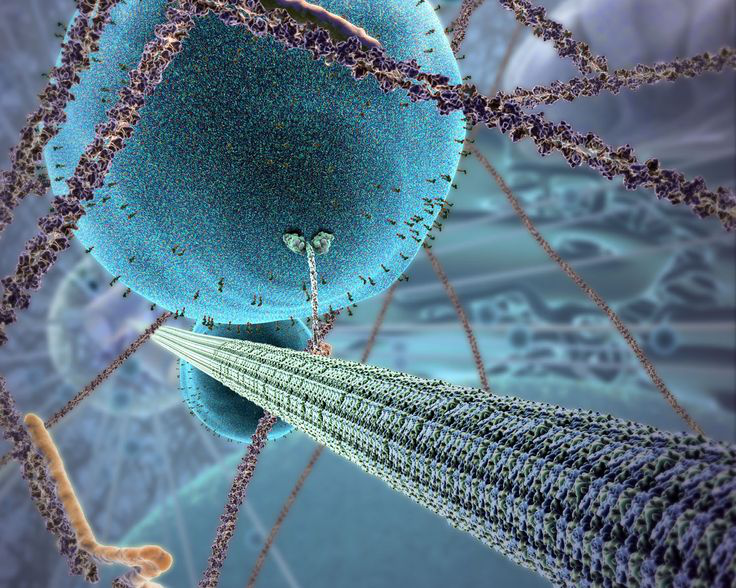
\includegraphics[width=0.7\textwidth]{kinesin_graphic}
  \caption{Kinesin-1 with cargo on microtubules	\cite{kinesin_graphic}}
  \label{fig:Kinesin}
\end{figure}
\end{titlepage}

\tableofcontents
\pagebreak

%------------------------
\section{Basics}

Proteins are the basis of every living organism. They perform all types of work inside the cells. In this experiment, the interaction of the cytoskeletal motor protein kinesin-1 with microtubule filaments is investigated at two different temperatures. Most of the following principles are described in the used script. \cite{script}

\subsection{Microtubules}

Microtubules are hollow polymer-cylinders. They are highly dynamic filaments, always shrinking or growing, which serve as tracks for active intercellular transport. Microtubules consists of tubulin subunits, which give the tubules a plus and minus end, which allow a directed transport. A picture of them can be seen in figure \ref{fig:Kinesin}. \\
In this experiment, the dynamic of the tubules is stopped by Taxol, which connects to the ends of them. The microtubules are labeled with rhodamine to allow red fluorescence.

\subsection{Kinesin-1}

Kinesin-1 is a motor protein which transports cargo around the cell. It consists of two identical, connected subunits which both have a head, a stalk and a tail, as can be seen in figure \ref{fig:Kinesin}. The head serves as motor, the tail as cargoholder. \\
The movement of kinesin-1 is accomplished through bipedal walk along microtubules: one head moves in front, the other stays connected to the microtubule. For each step, the kinesin-1 “consumes” one ATP-molecule to achieve the needed energy. In this way the protein manages to accomplish a velocity of 0.8\,$\mu m/s$. However, with a probability of 1\% both heads disconnect, resulting in a detachment of the microtubule after an average way length of 0.8\,$\mu m$.\\
In this experiment, the kinesin-1 proteins are labeled with GFP to provide green fluorescence. The used assay is a stepping assay, meaning that the kinesin-1 walk on the microtubules.

\subsection{Fluorescence microscopy}

To investigate the proteins fluorescence microscopy is used. The rhodamine and the GFP are excited by light: One of their electrons enters an excited orbital. This electron has the opposite spin of the remaining electron in the ground-state orbital. The molecules begin to vibrate and lose thermic energy in the process. After around 10\textsuperscript{-8} seconds the excited electron jumps back to the ground state and emits a photon. Because of the lost energy, the emitted photon has a larger wavelength then the absorbed one and can be distinguished from the laser light. Through this the tubules and proteins with the excited molecules can be observed.\\
To limit the fluorescing volume and gain a clear picture, Total Internal Reflection Fluorescence Microscopy is used. The exciting laser lights are totally reflected before they enter the object. However, an evanescent wave enters the object. Thus, only the first few microtubules and kinesin-1 are illuminated.

\section{Experimental procedure}

The movement of kinesin-1 has to be researched at two different temperatures: $25^\circ\text{C}$ and $37^\circ\text{C}$.
At first one prepares a flow-cell: two pieces of glass – one hydrophob, one hydrophil to provide a better flow of the liquids – are fused with 3 pieces of parafilm to form two channels, one as a backup. Then the channels are flushed with BRB80 – this is done after every flushing, to wash the channels, keep them wet and provide a good environment for the experiment. Then Anti-Tubulin antibodies, to bind the microtubules in the channels, and F127, to prevent the binding of the kinesin-1 with the glass, are put inside next. After this the microtubules, are flushed in. After a waiting time of around 1h the kinesin-1 final solution, which includes the kinesin-1, nutrients for both the microtubules and the kinesin-1 and ATP for the movement of the kinesin-1, is flushed in.

To see the behaviour the samples are researched with a TIRF-microscope with a magnification of 100x and a camera pixel-size of 16\,$\mu m\textsuperscript{2}$. At first a photo of the microtubules is taken at normal light, to determine the position of the microtubules. After this a 1000-frames video is taken under green laser light, to see the movement of the kinesin-1. The data-analysis is done using the FIESTA-program which is contributed. Here the lines of the microtubules are marked as can be seen in figure \ref{fig:marking} and, after the computer marked tracks of moving particles on this lines, for each temperature 200-500 recognizable tracks of the kinesin-1 are marked. The program calculates the velocity and run-length of this marked tracks.

\begin{figure}[!ht] 
  \centering
     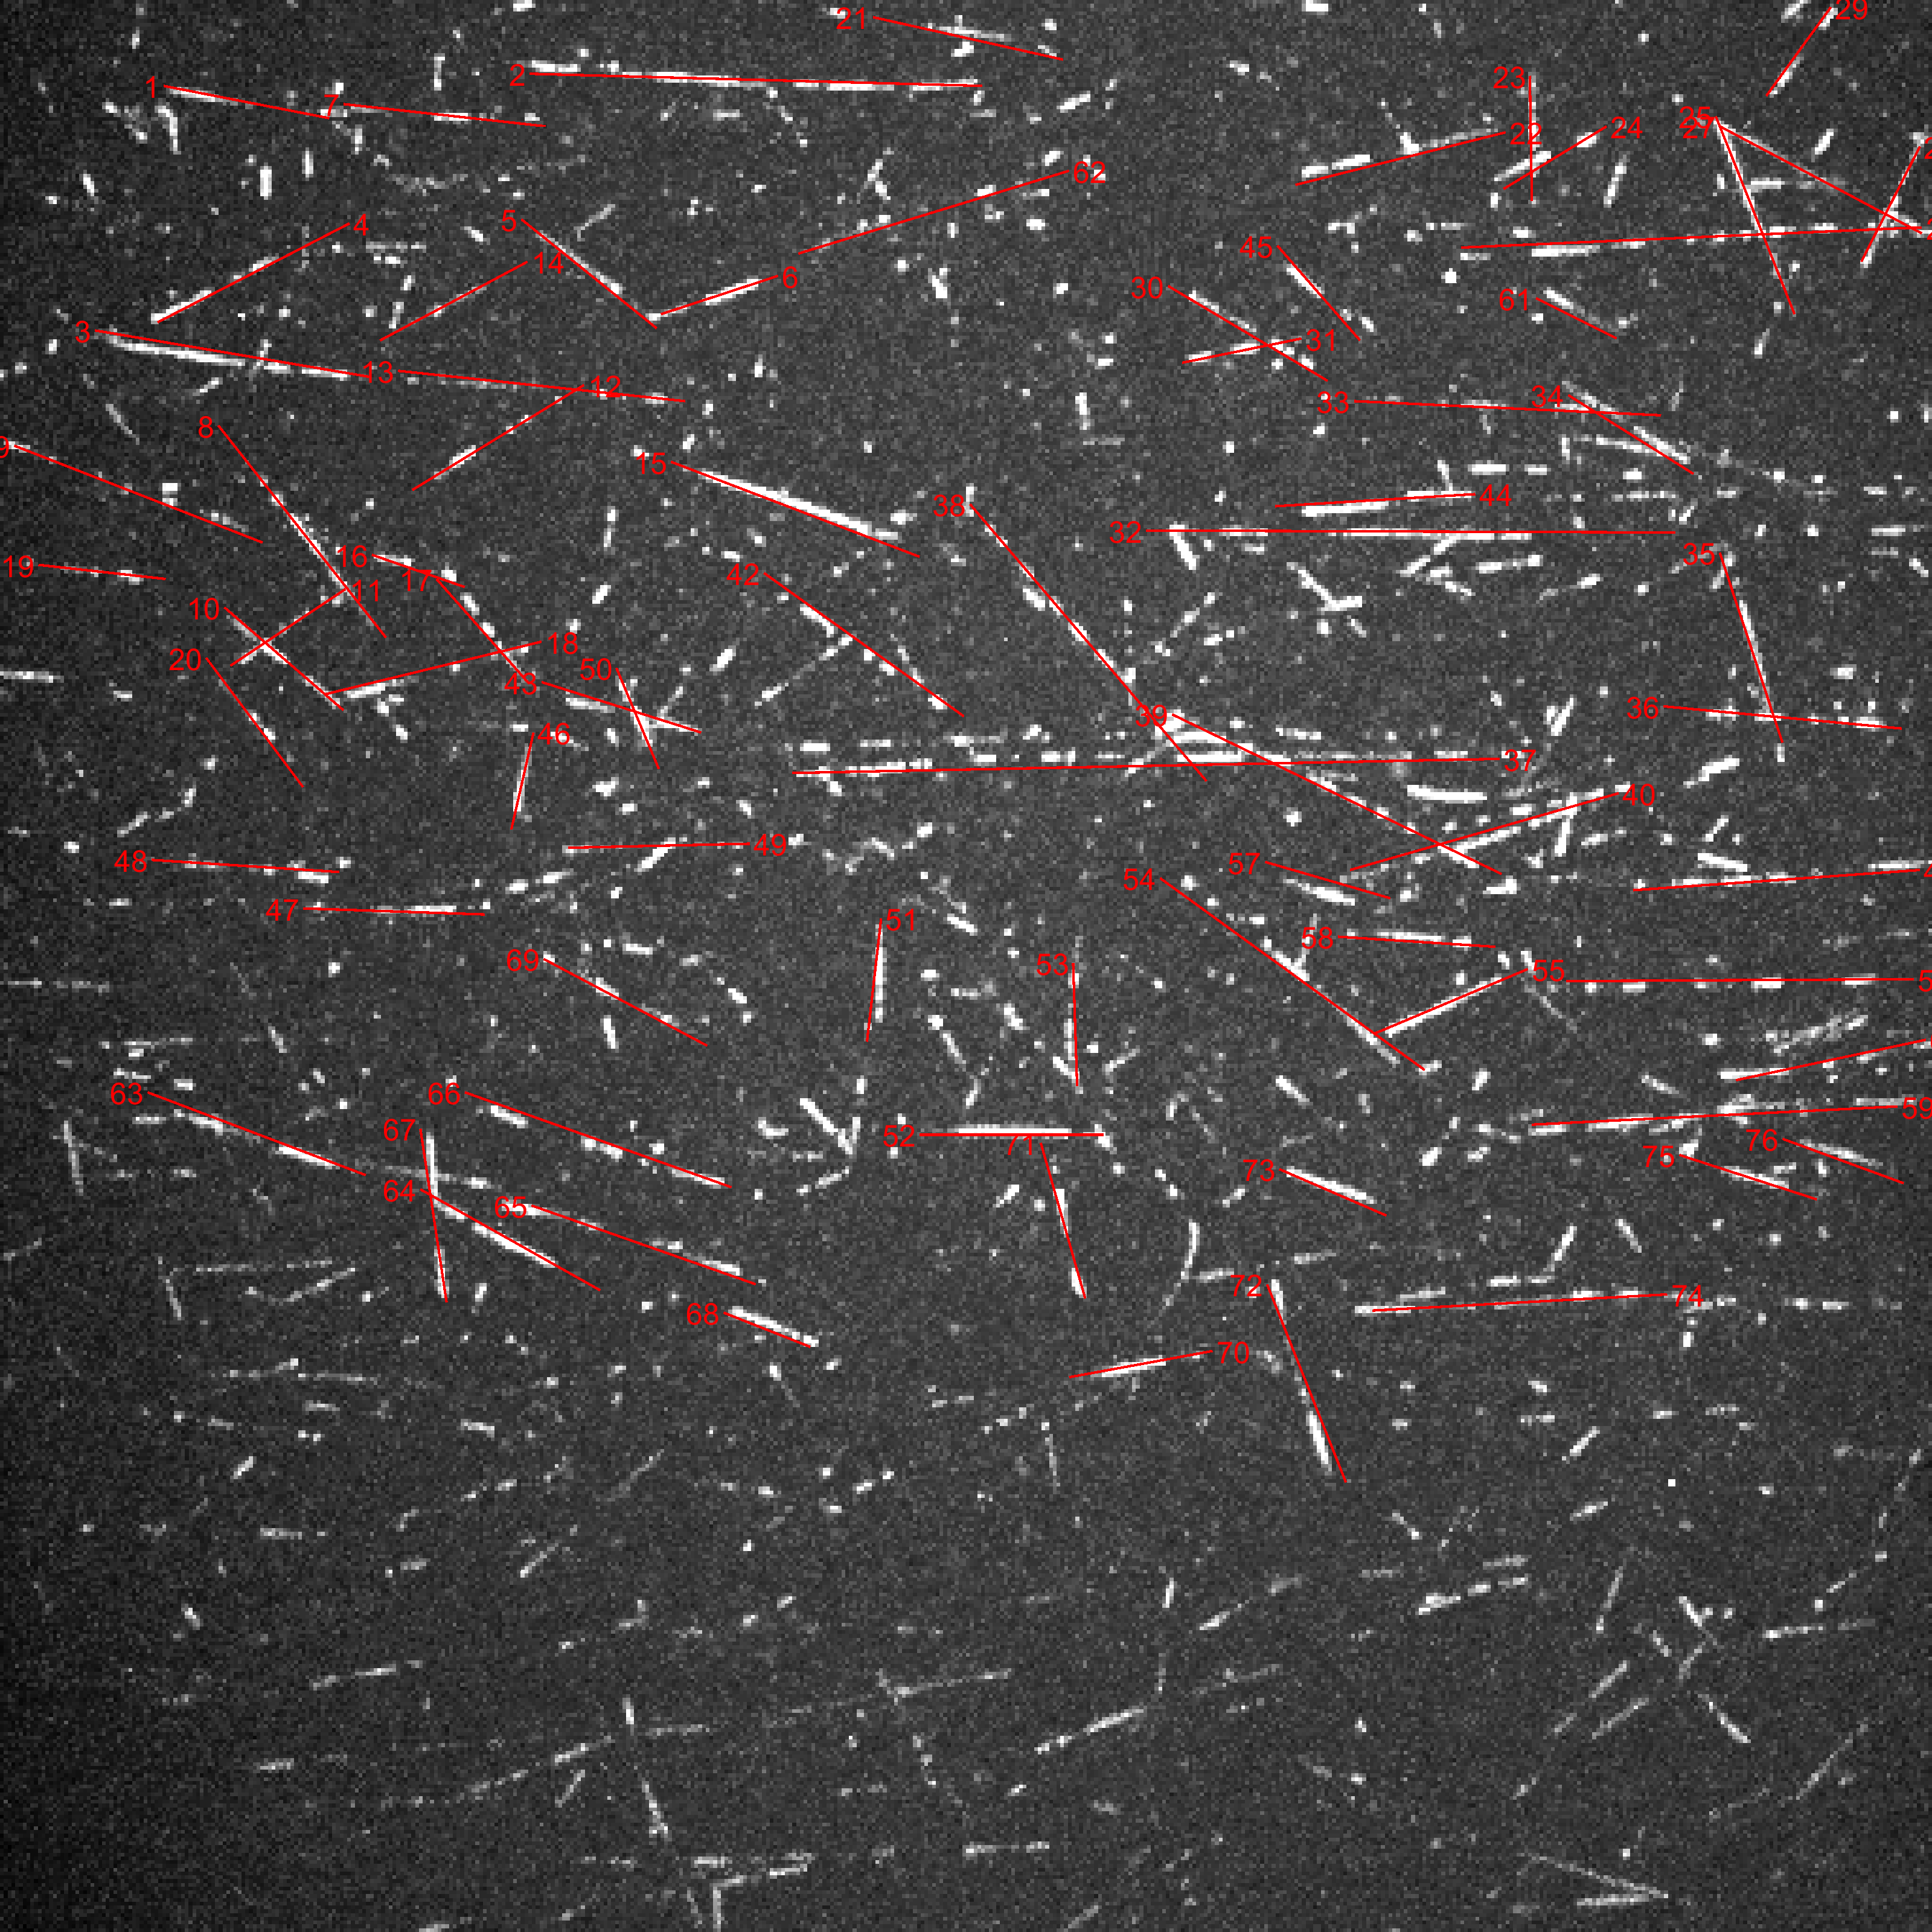
\includegraphics[width=0.7\textwidth]{kinesin_marking}
  \caption{Marking of microtubules in FIESTA for analysis}
  \label{fig:marking}
\end{figure}

\section{Data and analysis}

After the laserlight shone on the probes, the microtubules dissolved. This happened both for the main and the backup-channel of the flow-cell. Because time was short, the experiment couldn't be redone.
The reason for this problem was probably the kinesin-1 final solution, which contained nutrients and stabilizers, was tarnished, even though this solution was reproduced after the first failure. Because the second group, which did their experiment on the same day, had the same problem, it probably wasn't an experimentation error, but the basic liquids for the solution were tarnished. 
As we had no usable experimental data of ourselves, the following data-analysis is performed with data of another group. The extraction of the data by using FIESTA was performed by us. 

We acquired the following amount of movement incidents: 
\begin{align*}
25^\circ C \ : \ 546 \\
37^\circ C \ : \ 513
\end{align*}

\begin{figure}[htp] 
  \centering
     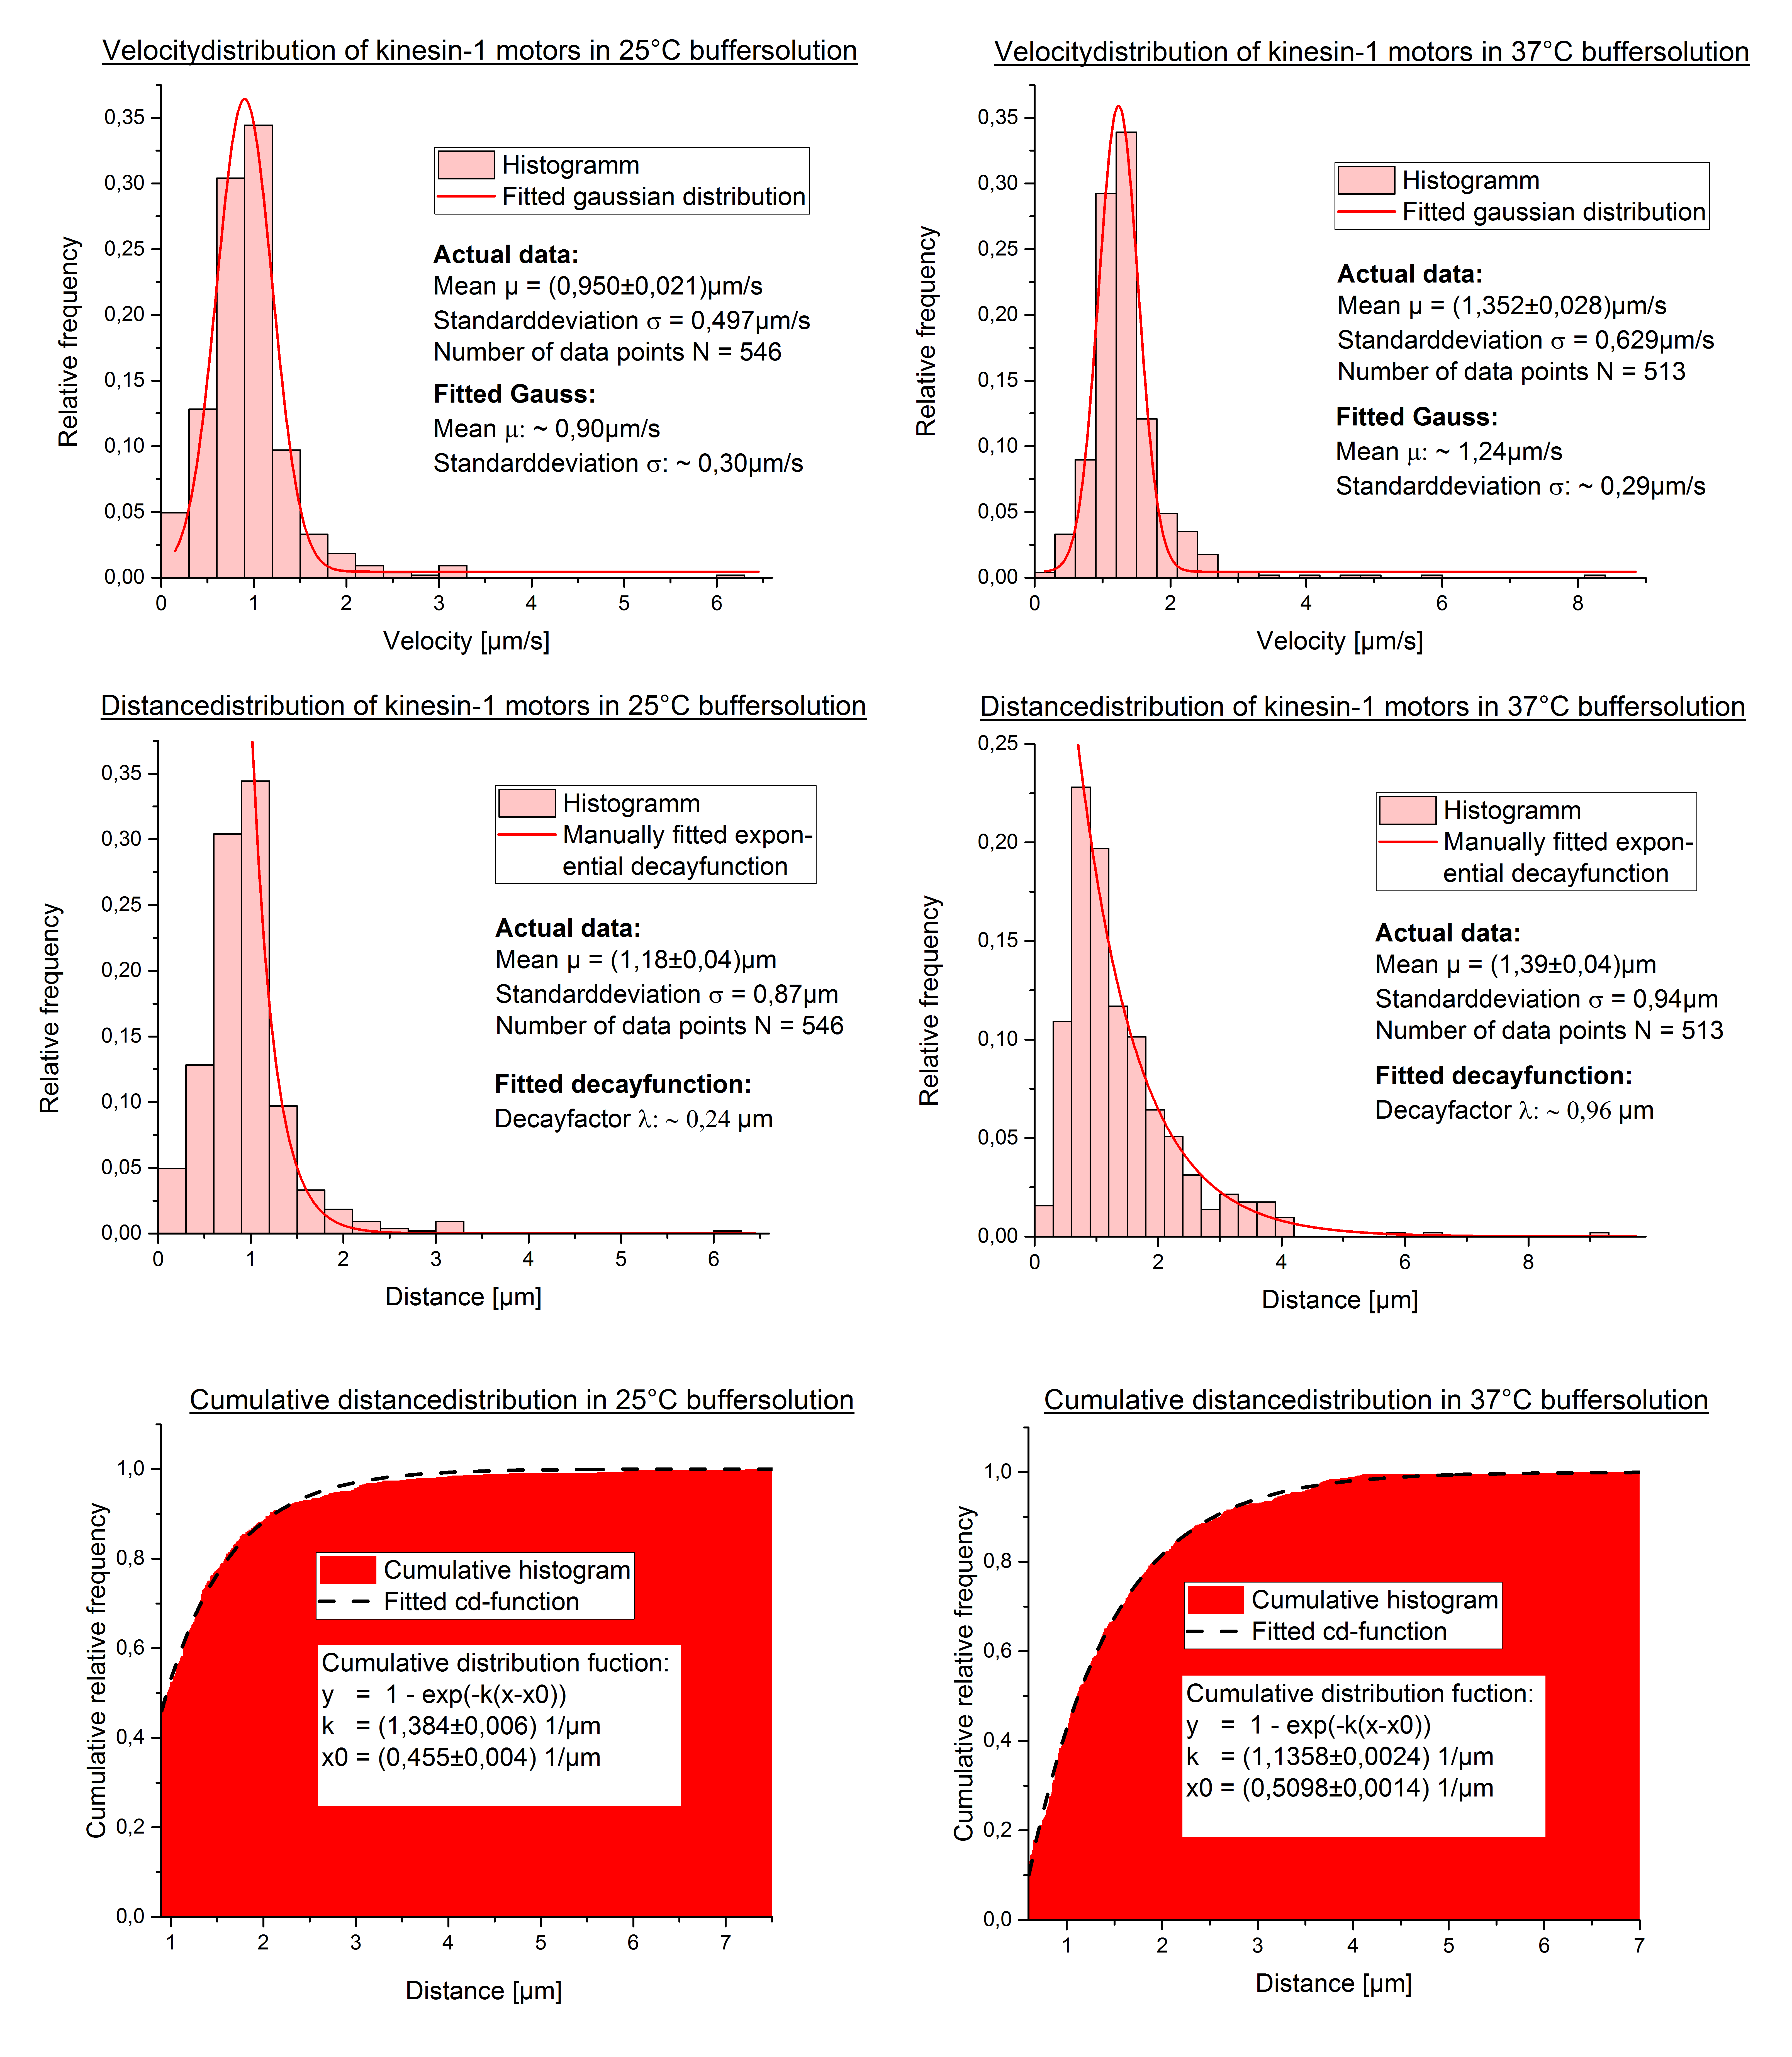
\includegraphics[width=1.0\textwidth]{all_diagrams.png}
  \caption{Chosen bin size: 0.3\,$\mu m/s$\\
	top-left: Normalized velocity of kinesin-1 at $25^\circ$ C; \\
	top-right: Normalized velocity of kinesin-1 at $37^\circ$ C; \\
	chosen bin size: 0.3\,$\mu m$ \\
	mid-left: Normalized run-length of kinesin-1 at $25^\circ$ C; \\
	mid-right: Normalized run-length of kinesin-1 at $37^\circ$ C; \\
	chosen bin size: 8\,$nm$ \\
	bottom-left: Cumulative run-length of kinesin-1 at $25^\circ$ C;\\
	bottom-right: Cumulative run-length of kinesin-1 at $37^\circ$ C}
  \label{fig:diagrams}
\end{figure}

\subsection{Velocity}

Histograms of the velocities are shown in figure \ref{fig:diagrams}. They resemble normal distributions, however, the performance of a Shapir-Wilk-test gives back a value of $W = 0.8$, which isn't enough to verify this claim. To make sure that this distributions are normal distributions, a bigger amount of incidents would be necessary. The calculated mean velocities with their standard deviations as errors are:
\begin{align*}
v _{25^\circ C} \ = \ (1.0 \ \pm \ 0.5) \, \mu m/s \\
v _{37^\circ C} \ = \ (1.4 \ \pm \ 0.6) \, \mu m/s
\end{align*}

These velocities seem to be higher than the literature value for kinesin-1 movement, which is 0.8\,$\mu m/s$. However, as the errors are very big, the literature values lie inside the error-range. A comparison of the two mean velocities leads to the claim, that the true mean velocities differ for $0.4\, \mu m/s$, the velocity of kinesin-1 in higher temperature seems to be higher. The performance of a Welch-test leads to a two-sided t-value of 0.956, which is bigger than 0.05. Therefore, the claim cannot be falsified. \\
TIRF-microscope is a very exact measurement, the gained pictures are very accurate, as can be seen in figure \ref{fig:marking}. Errors come mainly from the lack of sufficient incidents and the evaluation with FIESTA. Because the marking of microtubules and of kinesin-1-tracks was done manually, errors are inevitable. Normally, these errors should cancel each other statistically, however, as three different people did the evaluation of the data, this doesn't need to be the case. Another big error of the analysis should therefore be the lack of marked slow proteins: As very slow moving particles weren't marked, because they could be dead proteins or errors of the picture, very slow moving kinesin-1 are ignored.

\subsection{Run-length}

The histograms of the run-length can also be found in figure \ref{fig:diagrams}. These distributions can be fitted with an exponential fit. We fitted without using the first three bins for $25^\circ C$ and without using the first two bins for $37^\circ C$. The first bins aren't reliable, as the slowest moving kinesin-1 weren't marked, as explained above. The formula for the fit is:
\begin{align*}
y = a (1 - e^{-bx})^c
\end{align*}

The calculated mean run-lengths with their standard deviation as errors are:
\begin{align*}
l _{25^\circ C} \ = \ (1.2 \ \pm \ 0.9) \, \mu m \\
l _{37^\circ C} \ = \ (1.4 \ \pm \ 0.9) \, \mu m
\end{align*}

Again the claim is, that the true mean velocities differ for the same value than the measured mean velocities, in this case $l _{37^\circ C}$ is \(0.2\, \mu m\) bigger than $l _{25^\circ C}$. The Welch-test gives a two-sided t-value of 0.818. Because of this, the claim also cannot be neglected. 

To achieve an exacter value and lessen the error the cumulative distribution function for the run-lengths is now calculated and fitted. To grant a better visibility of the result, the chosen bin size is much smaller. The plots can be seen in figure \ref{fig:diagrams}. It can be seen, that the fit describes the graphs very precise, which supports our claim, that we can achieve a higher accuracy using this method. The formula for the fit is:
\begin{align*}
y = 1 - e^{-k(x - x0)}
\end{align*}

For this formula the mean value is calculated like this\cite{mean_cdf}:
\begin{align*}
\bar{x} = \frac{1}{k}
\end{align*}
And it's error with the Gauss' uncertainty propagation:
\begin{align*}
\Delta x = |\frac{-1}{k^2} \Delta k|
\end{align*}

Thus, the following values are achieved:
\begin{align*}
\bar{l} _{25^\circ C} \ = \ (0.7225 \ \pm \ 0.0031) \, \mu m \\
\bar{l} _{37^\circ C} \ = \ (0.8804 \ \pm \ 0.0019) \, \mu m
\end{align*}

Theses values are in the vicinity of the literature value for movement of kinesin-1 on microtubules, which is 0.8\,$\mu m$. 

\subsection{Interaction-time}

To achieve further insight in the dependence of kinesin-1 movement from temperature, the interaction-time of kinesin-1 with microtubules is also calculated, using the measured data. This is done using the following simple formula:
\begin{align*}
t_{interaction} = \frac{l_{run-length}}{v_{kinesin}}
\end{align*}
The error is calculated with Gauss:
\begin{align*}
\Delta t_{interaction} = \sqrt{(\frac{\Delta l_{run-length}}{v_{kinesin}})^2 + (- \frac{l_{run-length}}{v_{kinesin}^2} \Delta v_{kinesin})^2}
\end{align*}
Thus, the values for the interaction-time are:
\begin{align*}
t_{interaction; 25^\circ C} = (0.72 \pm 0.36)\,s
t_{interaction; 37^\circ C} = (0.6 \pm 0.4)\,s
\end{align*}
These values indicate, that, while velocity and run-length are rising with temperature, the interaction-time with the microtubules s shrinking. However, because of the big errors, further measurements would be needed to prove this.

\section{Discussion}

\begin{align*}
v_{25^\circ C} \ = \ (1.0 \ \pm \ 0.5) \, \mu m/s \\
v_{37^\circ C} \ = \ (1.4 \ \pm \ 0.6) \, \mu m/s
\end{align*}
\begin{align*}
\bar{l} _{25^\circ C} \ = \ (0.7225 \ \pm \ 0.0031) \, \mu m \\
\bar{l} _{37^\circ C} \ = \ (0.8804 \ \pm \ 0.0019) \, \mu m
\end{align*}
\begin{align*}
t_{interaction; 25^\circ C} = (0.72 \pm 0.36)\,s \\
t_{interaction; 37^\circ C} = (0.6 \pm 0.4)\,s
\end{align*}
The data indicate, that velocity and run-length are rising with temperature while the interaction-time is shrinking. To verify this claim, further measurement would be needed, as more incidents would lead to a lesser error for the velocity, which is the main reason for the big error of the interaction-time.

Problems of this experiment involve mainly the lack of sufficient incidents to achieve real normal distributions for the velocity and lessen the existing errors and the manual analysis with FIESTA, which doesn't allow to differentiate between dead kinesin-1, impurities in the probe and slow moving kinesin-1. \\
Our own experimental set-up also suffered from not-stabilized microtubules, either because of bad work or, more likely because remaking of the stabilization and nutrient-giving solution didn't make a difference and another group suffered from the same problem at the same time, the used materials were damaged.

\subsection{Conclusion}

In this experiment we managed to achieve data of the interaction of kinesin-1 with microtubules both at room- and at body-temperature. We saw, that kinesin-1 probably move faster and over longer distances at body-temperature, which is helpful for inner-cell transport, as the more distant regions, for example the axon terminals of neuron cells, are reached faster.  

%------------------------

\begin{thebibliography}{9}

\bibitem{script}
  http://www.bcube-dresden.de/fileadmin/www.bcube-dresden.de/uploads/diez/Versuch\_MMC\_WS2016\_Anleitung\_small.pdf
	03.11.2016
	12:00 o'clock

\bibitem{kinesin_graphic}
  http://ww1.prweb.com/prfiles/2009/09/08/140163/XVIVOHarvardKinesinMidView.jpg
	02.11.2016
	18:00 o'clock
	
\bibitem{mean_cdf}	
  https://en.wikipedia.org/wiki/Exponential\_distribution
	02.11.2016
	17:30 o'clock

\end{thebibliography}

\end{document}
